\documentclass{article}
\usepackage[utf8]{inputenc}
\usepackage{amsfonts}
\usepackage{graphicx}
\usepackage{pdfpages}
\usepackage{float}

\graphicspath{ {./figures/} }

\title{Unsupervised Sentiment Analysis}
\author{Lucas Rodrigues Pereira and Mathieu Pont\\\\directed by Mickael Febrissy and Lazhar Labiod\\\\Paris University, France}
\date{May 2019}

\begin{document}

\maketitle



\abstract{blablabla}



\section{Introduction}

Sentiment Analysis (or opinion mining) is the process of finding the sentiment of a document (text, audio etc.). In the simpler form the sentiment found is rather positive, negative or neutral, but it can be more complex like a rating (from 1 to 5 with 1 being the most negative and 5 the most positive, for example).

Unsupervised learning (or clustering) is the process of partitioning a dataset in different groups having similarities, without the help of an oracle (a "teacher" saying the answer, i.e. the real group of each data).

During our computer science master degree at Paris University we were asked
to do sentiment analysis on the "Scale Movie Review Dataset v1.0" [Pang et al., 2005] using unsupervised learning. This dataset is composed of 5006 movie reviews from 4 different authors. Each review has already it's own label but the goal of this work is to see what can do unsupervised learning on this kind of problem. The label is a rating like described upper (1 to 5 stars).



\section{Related Work}



\section{Preprocessing documents}

Some preprocessing are needed to correctly use the documents for sentiment analysis. The more different words we have, the more difficult it will be to classify documents. Therefore we want to remove words that are not important for the classification task. 

We search words that doesn't have any semantic values like the word \textit{"the"} or \textit{"you"} for example, we call this kind of words \textit{stop words}. We can also remove punctuation, numbers and put each word in lower case. Another preprocessing called \textit{lemmatization} tries to change each word into it's word stem. For example the word \textit{"gone"} will become \textit{"go"}. We removed the words that appears less than 10 times across all the documents, indeed if a word is very rare then it's probably not important.

The python library \textit{nltk} gives us a lot of tools to do this kind of preprocessing. After these preprocessings we finally had 9749 different words over all documents for \textbf{TODO} words before so we kept \textbf{TODO}\% of all the words.



\section{Encoding documents in vector format}

The first step to do sentiment analysis is to encode all documents in a vector format that will be used as input for a classification algorithm for example. 

One of the simplest encoding is the \textit{bag of words}, it's simply an histogram of the words present in each document. The output is a matrix \textbf{X} $\in \mathbb{R}^{n \times t}_{+}$ where \textit{n} is the number of documents and \textit{t} the total number of words within all documents. $x_{ij}$ is the number of times the word corresponding to the column \textit{j} appears in the document \textit{i}. We call this matrix the document/term matrix.

Another method, based on the \textit{bag of words}, is the \textit{TF-IDF score} that stands for \textit{Term Frequency and Inverse Document Frequency}. This score is computed for each word in each document. It gives us in output a matrix \textbf{X} with the same properties than with the \textit{bag of words} except that we multiply the frequency of the word in the document by a factor depending on the frequency of the word across all the documents like in equation \ref{eq:tf-idf}. 

\begin{equation}
x_{ij} = tf_{ij} \times \log\frac{N}{df_{j}}
\label{eq:tf-idf}
\end{equation}

Where $tf_{ij}$ is the frequency of word \textit{j} in document \textit{i}. \textit{N} the total number of documents. $df_{j}$ is the number of documents containing the word \textit{j}. Multiplying the second factor to the frequency of the word allows us to give more importance to word that are rare across all documents. Indeed words that occurs frequently across documents will not help us very much to discriminate them.

Finally we can apply L2 normalization to make each vector unit length, i.e. its norm equals 1. 

For our first experiments we used the \textit{TF-IDF} matrix with L2 normalization.



\section{Sentiment analysis experiments}

Here we use many unsupervised algorithms trying to find the correct class of each document.



\subsection{K-Means and Spherical K-Means}

The idea of these algorithms is to create \textit{k} clusters. Each of them gather documents by their similarities measured by a distance. K-Means uses Euclidean distance while Spherical K-Means uses cosinus distance.

The main difference is that Euclidean distance will regroup data points having similar coordinates whereas cosinus distance will regroup data points having their vector pointing in the same direction.

\paragraph{Elbow criterion.}
To find the value of \textit{k} we can use the elbow criterion. It implies to compute the algorithm for many values of \textit{k} and measure the percentage of variance explained by the clusters. For each \textit{k} we need to run the algorithm many times because the result depends on the initialization of the clusters which changes for each execution.

For a certain \textit{k} adding another cluster will not really help us in the data modeling, it will not add much to the variance explained. The behaviour expected is to see the first clusters adding a lot to the variance explained then the gain for each cluster added will drop and ideally we should see an angle in the graph.

\begin{figure}[H] 
\centering
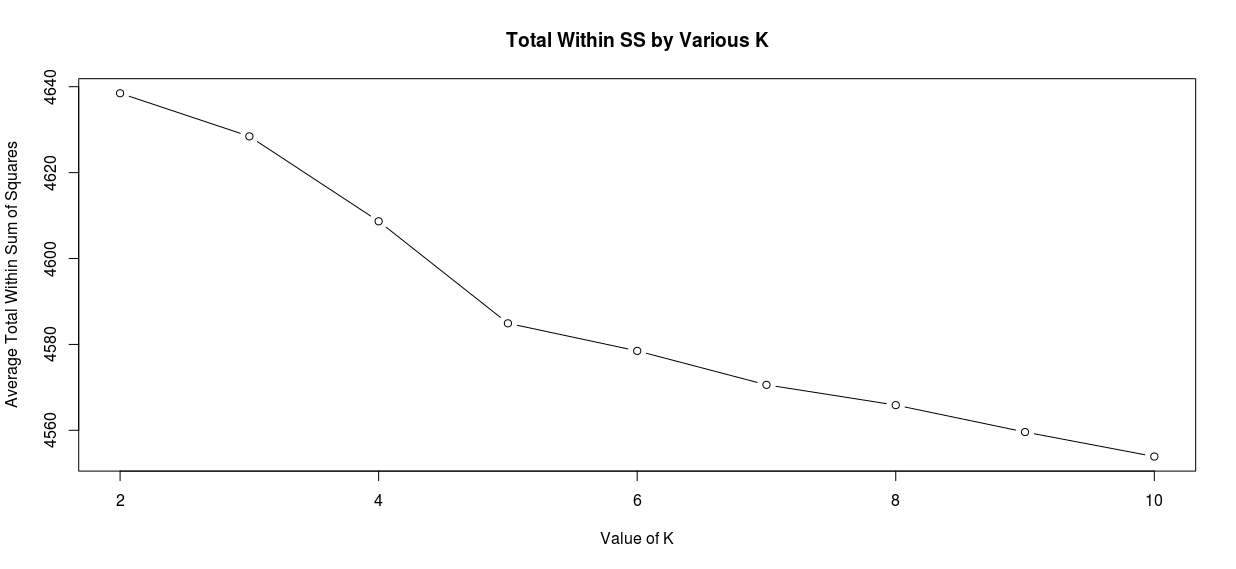
\includegraphics[width=\textwidth]{Kmeans_tf-idf-l2_elbow_criterion.png}
\caption{Elbow criterion for K-Means algorithm.}
\label{fig:elbow}
\end{figure}

We can see in figure \ref{fig:elbow} the elbow criterion for K-Means with the total within sum of squares as a measure. We can easily see an angle in the curve for the value \textit{k = 5}. This make sense because our documents are separated in 5 classes.

\paragraph{Documents clustering.}
Then we use the K-Means and Spherical K-Means to separate our documents in clusters.

We see at the top of figure \ref{fig:kmeans_skmeans} the real clusters, then the clusters found by K-Means and finally those found by Spherical K-Means. In the real clusters graph we can see four "staircase" composed of five "steps" each. Each staircase correspond to an author and each step to the reviews having a same rating.

\begin{figure}[H]
\centering
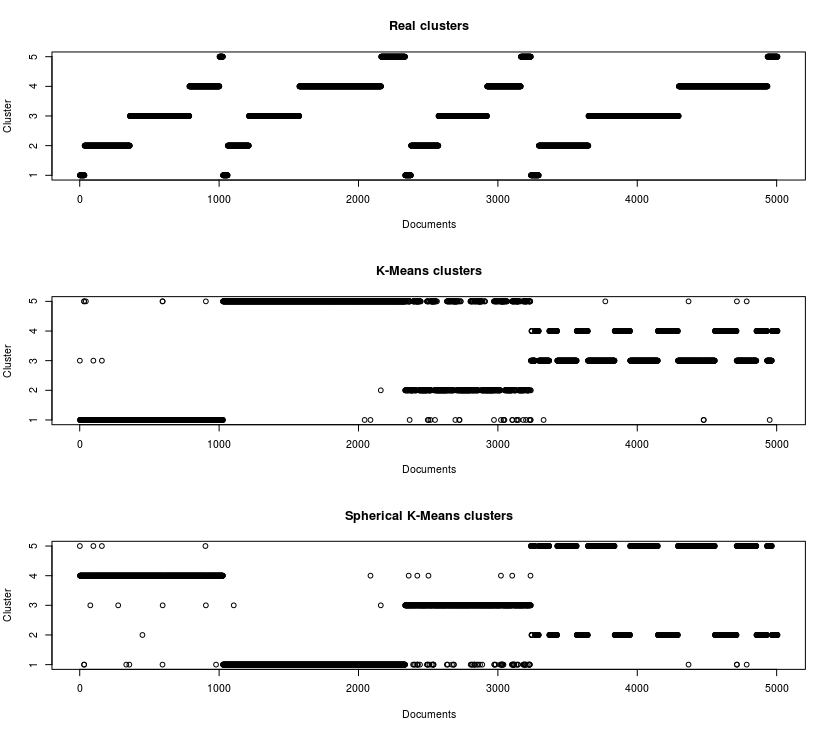
\includegraphics[width=\textwidth]{kmeans_and_skmeans.png}
\caption{Cluster of each document with K-Means.}
\label{fig:kmeans_skmeans}
\end{figure}

The clusters found by K-Means and Spherical K-Means are more or less the same. They both regroup the reviews of a same author in a same cluster. Instead of partitioning the documents according to their rating they were partitioned depending on their author. As we have four authors and five clusters the reviews of the last author were separated in two different clusters.

This result can be explained by the fact that the writing styles within authors have more in common than the writing styles for different authors giving the same rating. In other words the reviews of an author are more similar than the reviews having the same rating (according to the Euclidean and cosinus distance).
\\\\
To evaluate the clustering we use as metrics the Normalized Mutual Information (NMI) and Adjusted Rand Index (ARI) between the true distribution and the one found by the algorithms.

\begin{table}[H] \label{tab:kmeans_nmi_ari}
\centering
\begin{tabular}{|l|c|r|}
  \hline
  & NMI & ARI \\
  \hline
  K-Means & 0.023 & 0.016 \\
  Spherical K-Means & 0.026 & 0.020 \\
  \hline
\end{tabular}
\caption{NMI and ARI for K-Means and Spherical K-Means.}
\end{table}



\subsection{Other unsupervised algorithms}

We then try to use other unsupervised algorithms such as Deep Autoencoder and Latent Dirichlet Allocation (LDA).



\subsection{Other ways to represent documents}

We also try to represent the documents with other methods such as Doc2Vec [Le et al., 2014] and the Density Matrix Representation [Zhang et al., 2018] and then re-run the unsupervised algorithms on the dataset produced by these methods.

We've used a variant of the Density Matrix Representation, instead of only use the term frequency for the computation we used the \textit{TF-IDF} score normalized with L2 since this score seems to be better than the simple term frequency score.

The library \textit{gensym} was used for Doc2Vec, the Density Matrix Representation was implemented from scratch.

K-Means and Spherical K-Means produced the same results than with the \textit{TF-IDF} matrix with L2 normalization, the clusters corresponded to the authors of the documents was found instead of the rating.



\subsection{Use of external information: SentiWordNet}
After these results we have decided to add external information to help algorithms to correctly extract the sentiment of the reviews.

We found SentiWordNet [Baccianella et al., 2010], this is a dictionary composed of a lot of words (more than 150 000) and each of them is associated with two scores, each of them indicate how much the word is positive or negative. SentiWordNet founds 78\% (7604 in 9749 words) of the vocabulary of our documents.

Then, with the help of the SentiWordNet dictionary, we have made the matrix \textbf{S} $\in \mathbb{R}^{t \times 3}_{+}$ with \textit{t} the total number of words within all documents. Each word is associated with 3 scores, how much is a positive, negative and neutral word. A word is neutral if it doesn't have a positive or a negative score or if it's not found in the dictionary. We call this matrix the term/sentiment matrix.



\subsection{Variant of Word Co-Occurence Non-Negative Matrix Tri-Factorization (WC-NMTF)}

This method is based on Non-Negative Matrix Tri-Factorization (NMTF) [Long et al., 2005] et [Ding et al., 2006] which factorizes an input matrix \textbf{X} $\in \mathbb{R}^{n \times t}_{+}$ into three matrices \textbf{Z} $\in \mathbb{R}^{n \times g}_{+}$, \textbf{S} $\in \mathbb{R}^{g \times m}_{+}$ and \textbf{W} $\in \mathbb{R}^{t \times m}_{+}$ such that all matrices doesn't have any negative values and:

\begin{equation}
X \approx ZSW^{T}
\label{eq:nmf}
\end{equation}

\textbf{Z} plays the role of the cluster membership of each document if we have \textit{g} clusters. 

The Word Co-Occurence Non-Negative Matrix Tri-Factorization (WC-NMTF) [Salah et al., 2018] uses the same factorization but also factorizes an other matrix \textbf{M} $\in \mathbb{R}^{t \times t}_{+}$ into the matrices \textbf{W} $\in \mathbb{R}^{t \times m}_{+}$ and \textbf{Q} $\in \mathbb{R}^{t \times m}_{+}$ such that:

\begin{equation}
M \approx WQ^{T}
\label{eq:nmtf}
\end{equation}

WC-NMTF factorizes both \textbf{X} and \textbf{M}. Note that the same \textbf{W} matrix is used in equation \ref{eq:nmf} and \ref{eq:nmtf}.

In our case \textbf{X} is the document/term matrix. \textbf{W} is a term/term matrix also called the context matrix.



\section*{References}

\begin{list_type}  
\item [Pang et al., 2005] - Bo Pang and Lillian Lee. Seeing stars: Exploiting class relationships for sentiment categorization with respect to rating scales. 2005.
\item [Long et al., 2005] - Bo Long, Zhongfei (Mark) Zhang and Philip S. Yu. Co-clustering by Block Value Decomposition. 2005.
\item [Ding et al., 2006] - Chris Ding, Tao Li, Wei Peng Haesun Park. Orthogonal Nonnegative Matrix Tri-Factorizations for Clustering. 2006.
\item [Baccianella et al., 2010] - Stefano Baccianella, Andra Esuli,and Fabrizio Sebastiani. SENTIWORDNET 3.0: An Enhanced Lexical Resource for Sentiment Analysis and Opinion Mining. 2010.
\item [Le et al., 2014] - Quoc V. Le and Tomas Mikolov. Distributed Representations of Sentences and Documents. 2014.
\item [Salah et al., 2018] - Aghiles Salah, Melissa Ailem and Mohamed Nadif. Word Co-Occurrence Regularized Non-Negative Matrix Tri-Factorization for Text Data Co-Clustering. 2018.
\item [Zhang et al., 2018] - Yazhou Zhang, Dawei Song, Xiang Li and Peng Zhang. Unsupervised Sentiment Analysis
of Twitter Posts Using Density Matrix. 2018.
Representation.
\end{list_type}

\end{document}